% !TeX program = pdflatex
% !TeX root = main.tex
% Báo cáo nhóm Week 3 - CO2017. Biên dịch: cd docs/report/latex && latexmk -pdf main.tex
% Hình lấy thẳng từ figures/ ở gốc repo (do scripts/plot.py sinh ra).
% Mọi chỗ còn phải điền đều có chữ \todo{...} (in màu đỏ). Tìm "\todo" để thấy hết.
\documentclass[12pt, a4paper, oneside]{article}
\usepackage[utf8]{vietnam}
\usepackage[left=40mm, right=25mm, top=40mm, bottom=25mm]{geometry}
\usepackage{amsmath,amsfonts,amssymb}
\usepackage{indentfirst,enumitem}
\usepackage{graphicx}
\usepackage{setspace}
\usepackage{hyperref}
\usepackage{listings}
\usepackage{tabularx}
\usepackage{xcolor}
\usepackage{scrextend}
\usepackage{caption}
\usepackage{booktabs}
\usepackage{array}
\usepackage{fancyhdr}
\usepackage{float}
\usepackage[most]{tcolorbox}
\usepackage[T5]{fontenc}
\usepackage{mathptmx}
\usepackage{titlesec}
\usepackage{tikz}
\graphicspath{{figures/}{../../../figures/}}

\titleformat{\section}[block]
  {\centering\normalfont\fontsize{14pt}{16.8pt}\bfseries\MakeUppercase}
  {\thesection}{0.5em}{}
\titleformat{\subsection}[hang]{\normalfont\normalsize\bfseries}{\thesubsection}{0.5em}{}
\titleformat{\subsubsection}[hang]{\normalfont\normalsize\bfseries\itshape}{\thesubsubsection}{0.5em}{}

\captionsetup[table]{position=top, labelfont=bf, textfont=it, font=small, skip=5pt}
\captionsetup[figure]{position=bottom, labelfont=bf, textfont=it, font=small, skip=5pt}
\captionsetup[lstlisting]{labelformat=empty, labelsep=none, textfont=it, font=small}
\renewcommand{\figurename}{Hình}
\renewcommand{\tablename}{Bảng}

\hypersetup{colorlinks=true, linkcolor=black, urlcolor=blue!50!black,
  pdftitle={CO2017 Week 3 - Monte Carlo Pi}}

\changefontsizes{13pt}
\renewcommand\thesection{\arabic{section}.}
\renewcommand\thesubsection{\arabic{section}.\arabic{subsection}}
\setlength{\parindent}{1.25cm}

\pagestyle{fancy}
\renewcommand{\headrulewidth}{0pt}
\fancyhf{}
\cfoot{\thepage}
\setlength{\headheight}{14.94pt}

\definecolor{codegreen}{rgb}{0,0.6,0}
\definecolor{codegray}{rgb}{0.5,0.5,0.5}
\definecolor{codepurple}{rgb}{0.58,0,0.82}
\definecolor{backcolour}{rgb}{0.95,0.95,0.92}
\lstdefinestyle{mystyle}{backgroundcolor=\color{backcolour}, commentstyle=\color{codegreen},
  keywordstyle=\color{blue}, numberstyle=\tiny\color{codegray}, stringstyle=\color{codepurple},
  basicstyle=\ttfamily\footnotesize, breaklines=true, keepspaces=true, numbers=left,
  numbersep=5pt, showstringspaces=false, tabsize=4}
\lstset{style=mystyle}
%%%%%%%%%%%%%%%%%%%%%%%%%%%%%%%%%%%%%%%%%%%%%%%%%%%%%%%%%%%%%%%%%%%%%%%%%%%%%%%%%%%%%%%%%%%%%%%%%%%%%%%%%%%%%%%%%%%%%%%%%%%%%
% Verilog Code Style
%%%%%%%%%%%%%%%%%%%%%%%%%%%%%%%%%%%%%%%%%%%%%%%%%%%%%%%%%%%%%%%%%%%%%%%%%%%%%%%%%%%%%%%%%%%%%%%%%%%%%%%%%%%%%%%%%%%%%%%%%%%%%
\definecolor{verilogcommentcolor}{RGB}{104,180,104}
\definecolor{verilogkeywordcolor}{RGB}{49,49,255}
\definecolor{verilogsystemcolor}{RGB}{128,0,255}
\definecolor{verilognumbercolor}{RGB}{255,143,102}
\definecolor{verilogstringcolor}{RGB}{160,160,160}
\definecolor{verilogdefinecolor}{RGB}{128,64,0}
\definecolor{verilogoperatorcolor}{RGB}{0,0,128}

% Verilog style
\lstdefinestyle{prettyverilog}{
   language           = Verilog,
   commentstyle       = \color{verilogcommentcolor},
   alsoletter         = \$'0123456789\`,
   literate           = *{+}{{\verilogColorOperator{+}}}{1}%
                         {-}{{\verilogColorOperator{-}}}{1}%
                         {@}{{\verilogColorOperator{@}}}{1}%
                         {;}{{\verilogColorOperator{;}}}{1}%
                         {*}{{\verilogColorOperator{*}}}{1}%
                         {?}{{\verilogColorOperator{?}}}{1}%
                         {:}{{\verilogColorOperator{:}}}{1}%
                         {<}{{\verilogColorOperator{<}}}{1}%
                         {>}{{\verilogColorOperator{>}}}{1}%
                         {=}{{\verilogColorOperator{=}}}{1}%
                         {!}{{\verilogColorOperator{!}}}{1}%
                         {^}{{\verilogColorOperator{$\land$}}}{1}%
                         {|}{{\verilogColorOperator{|}}}{1}%
                         {=}{{\verilogColorOperator{=}}}{1}%
                         {[}{{\verilogColorOperator{[}}}{1}%
                         {]}{{\verilogColorOperator{]}}}{1}%
                         {(}{{\verilogColorOperator{(}}}{1}%
                         {)}{{\verilogColorOperator{)}}}{1}%
                         {,}{{\verilogColorOperator{,}}}{1}%
                         {.}{{\verilogColorOperator{.}}}{1}%
                         {~}{{\verilogColorOperator{$\sim$}}}{1}%
                         {\%}{{\verilogColorOperator{\%}}}{1}%
                         {\&}{{\verilogColorOperator{\&}}}{1}%
                         {\#}{{\verilogColorOperator{\#}}}{1}%
                         {\ /\ }{{\verilogColorOperator{\ /\ }}}{3}%
                         {\ _}{\ \_}{2}%
                        ,
   morestring         = [s][\color{verilogstringcolor}]{"}{"},%
   identifierstyle    = \color{black},
   vlogdefinestyle    = \color{verilogdefinecolor},
   vlogconstantstyle  = \color{verilognumbercolor},
   vlogsystemstyle    = \color{verilogsystemcolor},
   basicstyle         = \scriptsize\fontencoding{T1}\ttfamily,
   keywordstyle       = \bfseries\color{verilogkeywordcolor},
   numbers            = left,
   numbersep          = 10pt,
   tabsize            = 4,
   escapeinside       = {/*!}{!*/},
   upquote            = true,
   sensitive          = true,
   showstringspaces   = false, %without this there will be a symbol in the places where there is a space
   frame              = single
}


% This is shamelessly stolen and modified from:
% https://github.com/jubobs/sclang-prettifier/blob/master/sclang-prettifier.dtx
\makeatletter

% Language name
\newcommand\language@verilog{Verilog}
\expandafter\lst@NormedDef\expandafter\languageNormedDefd@verilog%
  \expandafter{\language@verilog}
  
% save definition of single quote for testing
\lst@SaveOutputDef{`'}\quotesngl@verilog
\lst@SaveOutputDef{``}\backtick@verilog
\lst@SaveOutputDef{`\$}\dollar@verilog

% Extract first character token in sequence and store in macro 
% firstchar@verilog, per http://tex.stackexchange.com/a/159267/21891
\newcommand\getfirstchar@verilog{}
\newcommand\getfirstchar@@verilog{}
\newcommand\firstchar@verilog{}
\def\getfirstchar@verilog#1{\getfirstchar@@verilog#1\relax}
\def\getfirstchar@@verilog#1#2\relax{\def\firstchar@verilog{#1}}

% Initially empty hook for lst
\newcommand\addedToOutput@verilog{}
\lst@AddToHook{Output}{\addedToOutput@verilog}

% The style used for constants as set in lstdefinestyle
\newcommand\constantstyle@verilog{}
\lst@Key{vlogconstantstyle}\relax%
   {\def\constantstyle@verilog{#1}}

% The style used for defines as set in lstdefinestyle
\newcommand\definestyle@verilog{}
\lst@Key{vlogdefinestyle}\relax%
   {\def\definestyle@verilog{#1}}

% The style used for defines as set in lstdefinestyle
\newcommand\systemstyle@verilog{}
\lst@Key{vlogsystemstyle}\relax%
   {\def\systemstyle@verilog{#1}}

% Counter used to check current character is a digit
\newcount\currentchar@verilog
  
% Processing macro
\newcommand\@ddedToOutput@verilog
{%
   % If we're in \lstpkg{}' processing mode...
   \ifnum\lst@mode=\lst@Pmode%
      % Save the first token in the current identifier to \@getfirstchar
      \expandafter\getfirstchar@verilog\expandafter{\the\lst@token}%
      % Check if the token is a backtick
      \expandafter\ifx\firstchar@verilog\backtick@verilog
         % If so, then this starts a define
         \let\lst@thestyle\definestyle@verilog%
      \else
         % Check if the token is a dollar
         \expandafter\ifx\firstchar@verilog\dollar@verilog
            % If so, then this starts a system command
            \let\lst@thestyle\systemstyle@verilog%
         \else
            % Check if the token starts with a single quote
            \expandafter\ifx\firstchar@verilog\quotesngl@verilog
               % If so, then this starts a constant without length
               \let\lst@thestyle\constantstyle@verilog%
            \else
               \currentchar@verilog=48
               \loop
                  \expandafter\ifnum%
                  \expandafter`\firstchar@verilog=\currentchar@verilog%
                     \let\lst@thestyle\constantstyle@verilog%
                     \let\iterate\relax%
                  \fi
                  \advance\currentchar@verilog by \@ne%
                  \unless\ifnum\currentchar@verilog>57%
               \repeat%
            \fi
         \fi
      \fi
      % ...but override by keyword style if a keyword is detected!
      %\lsthk@DetectKeywords% 
   \fi
}

% Add processing macro only if verilog
\lst@AddToHook{PreInit}{%
  \ifx\lst@language\languageNormedDefd@verilog%
    \let\addedToOutput@verilog\@ddedToOutput@verilog%
  \fi
}

% Colour operators in literate
\newcommand{\verilogColorOperator}[1]
{%
  \ifnum\lst@mode=\lst@Pmode\relax%
   {\bfseries\textcolor{verilogoperatorcolor}{#1}}%
  \else
    #1%
  \fi
}

\makeatother
%%%%%%%%%%%%%%%%%%%%%%%%%%%%%%%%%%%%%%%%%%%%%%%%%%%%%%%%%%%%%%%%%%%%%%%%%%%%%%%%%%%%%%%%%%%%%%%%%%%%%%%%%%%%%%%%%%%%%%%%%%%%%
% C/C++ Code Style
%%%%%%%%%%%%%%%%%%%%%%%%%%%%%%%%%%%%%%%%%%%%%%%%%%%%%%%%%%%%%%%%%%%%%%%%%%%%%%%%%%%%%%%%%%%%%%%%%%%%%%%%%%%%%%%%%%%%%%%%%%%%%
\definecolor{ccommentcolor}{RGB}{34,139,34}    % Xanh lá
\definecolor{ckeywordcolor}{RGB}{0,0,255}      % Xanh dương
\definecolor{cnumbercolor}{RGB}{9,134,88}      % Xanh ngọc
\definecolor{cstringcolor}{RGB}{163,21,21}     % Đỏ gạch
\definecolor{coperatorcolor}{RGB}{0,0,0}       % Đen

\lstdefinestyle{prettyc}{
   language           = C++,
   commentstyle       = \color{ccommentcolor}\itshape,
   alsoletter         = 0123456789,
   literate           = *{+}{{\cColorOperator{+}}}{1}%
                         {-}{{\cColorOperator{-}}}{1}%
                         {=}{{\cColorOperator{=}}}{1}%
                         {<}{{\cColorOperator{<}}}{1}%
                         {>}{{\cColorOperator{>}}}{1}%
                         {!}{{\cColorOperator{!}}}{1}%
                         {^}{{\cColorOperator{$\land$}}}{1}%
                         {|}{{\cColorOperator{|}}}{1}%
                         {\&}{{\cColorOperator{\&}}}{1}%
                         {~}{{\cColorOperator{$\sim$}}}{1},
   morestring         = [b]",
   morestring         = [b]',
   identifierstyle    = \color{black},
   cconstantstyle     = \color{cnumbercolor},
   basicstyle         = \scriptsize\fontencoding{T1}\ttfamily,
   keywordstyle       = \bfseries\color{ckeywordcolor},
   numbers            = left,
   numbersep          = 10pt,
   tabsize            = 4,
   escapeinside       = {/*!}{!*/},
   upquote            = true,
   sensitive          = true,
   showstringspaces   = false,
   frame              = single
}

\makeatletter
\newcommand\language@c{C++}
\expandafter\lst@NormedDef\expandafter\languageNormedDefd@c\expandafter{\language@c}
\newcommand\getfirstchar@c{}
\newcommand\getfirstchar@@c{}
\newcommand\firstchar@c{}
\def\getfirstchar@c#1{\getfirstchar@@c#1\relax}
\def\getfirstchar@@c#1#2\relax{\def\firstchar@c{#1}}
\newcommand\addedToOutput@c{}
\lst@AddToHook{Output}{\addedToOutput@c}
\newcommand\constantstyle@c{}
\lst@Key{cconstantstyle}\relax{\def\constantstyle@c{#1}}
\newcount\currentchar@c
\newcommand\@ddedToOutput@c
{%
   \ifnum\lst@mode=\lst@Pmode%
      \expandafter\getfirstchar@c\expandafter{\the\lst@token}%
      \currentchar@c=48
      \loop
         \expandafter\ifnum%
         \expandafter`\firstchar@c=\currentchar@c%
            \let\lst@thestyle\constantstyle@c%
            \let\iterate\relax%
         \fi
         \advance\currentchar@c by \@ne%
         \unless\ifnum\currentchar@c>57%
      \repeat%
   \fi
}
\lst@AddToHook{PreInit}{%
  \ifx\lst@language\languageNormedDefd@c%
    \let\addedToOutput@c\@ddedToOutput@c%
  \fi
}
\newcommand{\cColorOperator}[1]{\ifnum\lst@mode=\lst@Pmode\relax{\bfseries\textcolor{coperatorcolor}{#1}}\else#1\fi}
\makeatother

%%%%%%%%%%%%%%%%%%%%%%%%%%%%%%%%%%%%%%%%%%%%%%%%%%%%%%%%%%%%%%%%%%%%%%%%%%%%%%%%%%%%%%%%%%%%%%%%%%%%%%%%%%%%%%%%%%%%%%%%%%%%%
% Python Code Style
%%%%%%%%%%%%%%%%%%%%%%%%%%%%%%%%%%%%%%%%%%%%%%%%%%%%%%%%%%%%%%%%%%%%%%%%%%%%%%%%%%%%%%%%%%%%%%%%%%%%%%%%%%%%%%%%%%%%%%%%%%%%%
\definecolor{pythoncommentcolor}{RGB}{34,139,34}  % Xanh lá
\definecolor{pythonkeywordcolor}{RGB}{0,0,255}    % Xanh dương
\definecolor{pythonnumbercolor}{RGB}{9,134,88}    % Xanh ngọc
\definecolor{pythonstringcolor}{RGB}{163,21,21}   % Đỏ gạch
\definecolor{pythonoperatorcolor}{RGB}{0,0,0}     % Đen

\lstdefinestyle{prettypython}{
   language           = Python,
   commentstyle       = \color{pythoncommentcolor}\itshape,
   alsoletter         = 0123456789,
   literate           = *{+}{{\pythonColorOperator{+}}}{1}%
                         {-}{{\pythonColorOperator{-}}}{1}%
                         {=}{{\pythonColorOperator{=}}}{1}%
                         {<}{{\pythonColorOperator{<}}}{1}%
                         {>}{{\pythonColorOperator{>}}}{1}%
                         {!}{{\pythonColorOperator{!}}}{1}%
                         {^}{{\pythonColorOperator{$\land$}}}{1}%
                         {|}{{\pythonColorOperator{|}}}{1}%
                         {\&}{{\pythonColorOperator{\&}}}{1}%
                         {~}{{\pythonColorOperator{$\sim$}}}{1},
   morestring         = [b]",
   morestring         = [b]',
   identifierstyle    = \color{black},
   pythonconstantstyle = \color{pythonnumbercolor},
   basicstyle         = \scriptsize\fontencoding{T1}\ttfamily,
   keywordstyle       = \bfseries\color{pythonkeywordcolor},
   numbers            = left,
   numbersep          = 10pt,
   tabsize            = 4,
   escapeinside       = {/*!}{!*/},
   upquote            = true,
   sensitive          = true,
   showstringspaces   = false,
   frame              = single
}

\makeatletter
\newcommand\language@python{Python}
\expandafter\lst@NormedDef\expandafter\languageNormedDefd@python\expandafter{\language@python}
\newcommand\getfirstchar@python{}
\newcommand\getfirstchar@@python{}
\newcommand\firstchar@python{}
\def\getfirstchar@python#1{\getfirstchar@@python#1\relax}
\def\getfirstchar@@python#1#2\relax{\def\firstchar@python{#1}}
\newcommand\addedToOutput@python{}
\lst@AddToHook{Output}{\addedToOutput@python}
\newcommand\constantstyle@python{}
\lst@Key{pythonconstantstyle}\relax{\def\constantstyle@python{#1}}
\newcount\currentchar@python
\newcommand\@ddedToOutput@python
{%
   \ifnum\lst@mode=\lst@Pmode%
      \expandafter\getfirstchar@python\expandafter{\the\lst@token}%
      \currentchar@python=48
      \loop
         \expandafter\ifnum%
         \expandafter`\firstchar@python=\currentchar@python%
            \let\lst@thestyle\constantstyle@python%
            \let\iterate\relax%
         \fi
         \advance\currentchar@python by \@ne%
         \unless\ifnum\currentchar@python>57%
      \repeat%
   \fi
}
\lst@AddToHook{PreInit}{%
  \ifx\lst@language\languageNormedDefd@python%
    \let\addedToOutput@python\@ddedToOutput@python%
  \fi
}
\newcommand{\pythonColorOperator}[1]{\ifnum\lst@mode=\lst@Pmode\relax{\bfseries\textcolor{pythonoperatorcolor}{#1}}\else#1\fi}
\makeatother

%%%%%%%%%%%%%%%%%%%%%%%%%%%%%%%%%%%%%%%%%%%%%%%%%%%%%%%%%%%%%%%%%%%%%%%%%%%%%%%%%%%%%%%%%%%%%%%%%%%%%%%%%%%%%%%%%%%%%%%%%%%%%
% Matlab Code Style
%%%%%%%%%%%%%%%%%%%%%%%%%%%%%%%%%%%%%%%%%%%%%%%%%%%%%%%%%%%%%%%%%%%%%%%%%%%%%%%%%%%%%%%%%%%%%%%%%%%%%%%%%%%%%%%%%%%%%%%%%%%%%
\definecolor{matlabcommentcolor}{RGB}{34,139,34}   % Xanh lá đậm chuẩn MATLAB
\definecolor{matlabkeywordcolor}{RGB}{0,0,255}     % Xanh dương chuẩn
\definecolor{matlabstringcolor}{RGB}{160,32,240}   % Tím đặc trưng cho chuỗi
\definecolor{matlabnumbercolor}{RGB}{0,0,0}        % Đen cho số
\definecolor{matlaboperatorcolor}{RGB}{0,0,0}      % Đen cho toán tử

\lstdefinestyle{prettymatlab}{
   language           = Matlab,
   commentstyle       = \color{matlabcommentcolor}\itshape,
   alsoletter         = 0123456789,
   literate           = *{+}{{\matlabColorOperator{+}}}{1}%
                         {-}{{\matlabColorOperator{-}}}{1}%
                         {=}{{\matlabColorOperator{=}}}{1}%
                         {<}{{\matlabColorOperator{<}}}{1}%
                         {>}{{\matlabColorOperator{>}}}{1}%
                         {!}{{\matlabColorOperator{!}}}{1}%
                         {^}{{\matlabColorOperator{$\land$}}}{1}%
                         {|}{{\matlabColorOperator{|}}}{1}%
                         {\&}{{\matlabColorOperator{\&}}}{1}%
                         {~}{{\matlabColorOperator{$\sim$}}}{1},
   morestring         = [b]', % MATLAB chỉ dùng nháy đơn cho chuỗi (char array)
   morestring         = [b]", % Hỗ trợ nháy kép cho String (bản MATLAB mới)
   identifierstyle    = \color{black},
   matlabconstantstyle = \color{matlabnumbercolor},
   basicstyle         = \scriptsize\fontencoding{T1}\ttfamily,
   keywordstyle       = \color{matlabkeywordcolor}, 
   numbers            = left,
   numbersep          = 10pt,
   tabsize            = 4,
   escapeinside       = {/*!}{!*/},
   upquote            = true,
   sensitive          = true,
   showstringspaces   = false,
   frame              = single
}

\makeatletter
\newcommand\language@matlab{Matlab}
\expandafter\lst@NormedDef\expandafter\languageNormedDefd@matlab\expandafter{\language@matlab}
\newcommand\getfirstchar@matlab{}
\newcommand\getfirstchar@@matlab{}
\newcommand\firstchar@matlab{}
\def\getfirstchar@matlab#1{\getfirstchar@@matlab#1\relax}
\def\getfirstchar@@matlab#1#2\relax{\def\firstchar@matlab{#1}}
\newcommand\addedToOutput@matlab{}
\lst@AddToHook{Output}{\addedToOutput@matlab}
\newcommand\constantstyle@matlab{}
\lst@Key{matlabconstantstyle}\relax{\def\constantstyle@matlab{#1}}
\newcount\currentchar@matlab
\newcommand\@ddedToOutput@matlab
{%
   \ifnum\lst@mode=\lst@Pmode%
      \expandafter\getfirstchar@matlab\expandafter{\the\lst@token}%
      \currentchar@matlab=48
      \loop
         \expandafter\ifnum%
         \expandafter`\firstchar@matlab=\currentchar@matlab%
            \let\lst@thestyle\constantstyle@matlab%
            \let\iterate\relax%
         \fi
         \advance\currentchar@matlab by \@ne%
         \unless\ifnum\currentchar@matlab>57%
      \repeat%
   \fi
}
\lst@AddToHook{PreInit}{%
  \ifx\lst@language\languageNormedDefd@matlab%
    \let\addedToOutput@matlab\@ddedToOutput@matlab%
  \fi
}
\newcommand{\matlabColorOperator}[1]{\ifnum\lst@mode=\lst@Pmode\relax{\textcolor{matlaboperatorcolor}{#1}}\else#1\fi}
\makeatother

\newcommand{\todo}[1]{\textcolor{red}{\textbf{[TODO: #1]}}}
\newcommand{\code}[1]{\texttt{#1}}

\begin{document}
% =============================================================================
% TRANG BÌA
% =============================================================================
\begin{titlepage}
\begin{tikzpicture}[remember picture,overlay,inner sep=0,outer sep=0]
  \draw[blue!70!black,line width=4pt] ([xshift=-1.5cm,yshift=-2cm]current page.north east) coordinate (A)--([xshift=3cm,yshift=-2cm]current page.north west) coordinate(B)--([xshift=3cm,yshift=2cm]current page.south west) coordinate (C)--([xshift=-1.5cm,yshift=2cm]current page.south east) coordinate(D)--cycle;
  \draw ([yshift=0.5cm,xshift=-0.5cm]A)-- ([yshift=0.5cm,xshift=0.5cm]B)--([yshift=-0.5cm,xshift=0.5cm]B) --([yshift=-0.5cm,xshift=-0.5cm]B)--([yshift=0.5cm,xshift=-0.5cm]C)--([yshift=0.5cm,xshift=0.5cm]C)--([yshift=-0.5cm,xshift=0.5cm]C)-- ([yshift=-0.5cm,xshift=-0.5cm]D)--([yshift=0.5cm,xshift=-0.5cm]D)--([yshift=0.5cm,xshift=0.5cm]D)--([yshift=-0.5cm,xshift=0.5cm]A)--([yshift=-0.5cm,xshift=-0.5cm]A)--([yshift=0.5cm,xshift=-0.5cm]A);
  \draw ([yshift=-0.3cm,xshift=0.3cm]A)-- ([yshift=-0.3cm,xshift=-0.3cm]B)--([yshift=0.3cm,xshift=-0.3cm]B) --([yshift=0.3cm,xshift=0.3cm]B)--([yshift=-0.3cm,xshift=0.3cm]C)--([yshift=-0.3cm,xshift=-0.3cm]C)--([yshift=0.3cm,xshift=-0.3cm]C)-- ([yshift=0.3cm,xshift=0.3cm]D)--([yshift=-0.3cm,xshift=0.3cm]D)--([yshift=-0.3cm,xshift=-0.3cm]D)--([yshift=0.3cm,xshift=-0.3cm]A)--([yshift=0.3cm,xshift=0.3cm]A)--([yshift=-0.3cm,xshift=0.3cm]A);
\end{tikzpicture}
\begin{center}
  \vspace{7pt}\textbf{ĐẠI HỌC QUỐC GIA THÀNH PHỐ HỒ CHÍ MINH}

  \vspace{7pt}TRƯỜNG ĐẠI HỌC BÁCH KHOA

  \vspace{7pt}KHOA KHOA HỌC VÀ KỸ THUẬT MÁY TÍNH
\end{center}
\vspace{10pt}
\begin{center}
\includegraphics[scale=0.25]{HCMUT.png}\end{center}
\vspace{10pt}
\begin{center}
  \fontsize{18pt}{20pt}\selectfont\textbf{BÁO CÁO BÀI TẬP NHÓM TUẦN 3}

  \vspace{6pt}
  \fontsize{15pt}{17pt}\selectfont\textbf{HỆ ĐIỀU HÀNH (CO2017)}
\end{center}
\begin{center}
  \fontsize{15pt}{18pt}\selectfont
  \textbf{ĐỀ TÀI: THỰC HÀNH ĐA LUỒNG TỐT\\QUA BÀI TOÁN ƯỚC LƯỢNG $\pi$ BẰNG MONTE CARLO}
\end{center}
\begin{center}
  \vspace{12pt}\textbf{Lớp: \todo{Lxx} -- Nhóm: \todo{xx}}

  \vspace{4pt}\textbf{GVHD: \todo{tên giảng viên}}
\end{center}
\vspace{4pt}
\begin{center}
\small\renewcommand{\arraystretch}{1.15}
\begin{tabular}{|c|l|c|}
\hline
\textbf{MSSV} & \textbf{Họ và tên} & \textbf{Việc} \\ \hline
\todo{MSSV} & \todo{Họ tên} (longquawns) & 1 \\ \hline
\todo{MSSV} & \todo{Họ tên} (AnhTu97ccmk) & 2 \\ \hline
\todo{MSSV} & \todo{Họ tên} (Hungluu1702) & 3 \\ \hline
\todo{MSSV} & \todo{Họ tên} (ggg-maker-pixel) & 4 \\ \hline
2452081 & Phạm Tuấn Anh (EigenKai) & 5 \\ \hline
\end{tabular}
\end{center}
\vfill
\centerline{\bf Thành phố Hồ Chí Minh, tháng 11 năm 2026}
\vspace{1cm}
\end{titlepage}

% =============================================================================
% PHÂN CÔNG
% =============================================================================
\newpage
\setstretch{1.3}
\section*{BẢNG PHÂN CÔNG NHIỆM VỤ}
\addcontentsline{toc}{section}{BẢNG PHÂN CÔNG NHIỆM VỤ}

Nhóm làm việc trên một repository chung, mỗi thay đổi đi qua một pull request và được review trước khi merge:
\url{https://github.com/PTAxHVA/os-week3-monte-carlo-pi}.

\begin{table}[H]
\centering
\renewcommand{\arraystretch}{1.5}
\renewcommand{\tabularxcolumn}[1]{m{#1}}
\begin{tabularx}{\textwidth}{|l|X|c|}
\hline
\textbf{Thành viên} & \multicolumn{1}{c|}{\textbf{Công việc}} & \textbf{Tỉ lệ} \\ \hline
\todo{Họ tên} (Việc 1) & \code{common.h} (giao ước chung), Approach 1, \code{Makefile}, README, ghép và nộp bài & 100\% \\ \hline
\todo{Họ tên} (Việc 2) & Approach 2 (biến đếm cục bộ, map--reduce); phân tích A, B, C, thí nghiệm 6.2 & 100\% \\ \hline
\todo{Họ tên} (Việc 3) & Approach 3 (mutex, tham số $k$); phân tích D, E, thí nghiệm 6.1, 6.3 & 100\% \\ \hline
\todo{Họ tên} (Việc 4) & Chạy toàn bộ phép đo trên máy đo chung, xuất số liệu và đồ thị & 100\% \\ \hline
Phạm Tuấn Anh (Việc 5) & Review mọi pull request, script đo và vẽ, thí nghiệm độ chính xác, viết báo cáo & 100\% \\ \hline
\end{tabularx}
\end{table}

\newpage
\renewcommand{\contentsname}{\centering MỤC LỤC}
\tableofcontents
\newpage
\renewcommand{\listfigurename}{\centering DANH SÁCH HÌNH}
\listoffigures
\renewcommand{\listtablename}{\centering DANH SÁCH BẢNG}
\listoftables

% =============================================================================
\newpage
\section{Mục tiêu}
Bài tập ước lượng $\pi$ bằng phương pháp Monte Carlo theo ba cách: một luồng, nhiều luồng với biến đếm cục bộ, và nhiều luồng dùng chung một biến đếm có khoá mutex. Bài toán $\pi$ chỉ là phương tiện. Thứ cần quan sát là:
\begin{itemize}
  \item thực thi song song cải thiện hiệu năng tới đâu, và vì sao dừng lại;
  \item chi phí của đồng bộ hoá và giao tiếp giữa các luồng;
  \item cách thiết kế chương trình đa luồng đúng;
  \item hành vi đo được liên hệ thế nào với bộ định thời của hệ điều hành và giới hạn phần cứng.
\end{itemize}

% =============================================================================
\section{Phương pháp}
\subsection{Ước lượng $\pi$ bằng Monte Carlo}
Lấy điểm $(x,y)$ ngẫu nhiên đều trong hình vuông $[0,1]^2$. Điểm nằm trong phần tư hình tròn bán kính 1 khi $x^2+y^2\le 1$. Phần tư hình tròn chiếm $\pi/4$ diện tích hình vuông, nên
\begin{equation}
  \pi \approx 4\cdot\frac{\text{số điểm trong hình tròn}}{\text{tổng số điểm}}.
\end{equation}
Đề bài vẽ hình trên $[-1,1]^2$ với cả hình tròn; tỉ lệ diện tích vẫn là $\pi/4$ nên hai cách cho cùng một ước lượng. Với $n$ điểm, sai số chuẩn của ước lượng là
\begin{equation}
  \sigma_{\hat\pi} = 4\sqrt{\frac{p(1-p)}{n}} \approx \frac{1{,}642}{\sqrt n}, \qquad p=\frac{\pi}{4},
  \label{eq:se}
\end{equation}
khoảng $5{,}2\cdot10^{-4}$ khi $n=10^7$.

\subsection{Môi trường đo}
Mọi phép đo thời gian chạy trên \textbf{một máy duy nhất} (yêu cầu của giảng viên), lấy từ \code{results/machine.txt}.

\begin{table}[H]
\centering
\caption{Máy đo}
\label{tab:machine}
\begin{tabularx}{\textwidth}{lX}
\toprule
Máy & Máy ảo VMware trên laptop AMD Ryzen 5 7235HS (4 nhân / 8 luồng) \\
CPU cấp cho máy ảo & 4 vCPU (1 socket $\times$ 4 nhân, 1 luồng mỗi nhân), \code{nproc} = 4 \\
Hệ điều hành & Ubuntu, nhân Linux 7.0.0-38-generic, x86\_64 \\
Trình biên dịch & gcc 15.2.0, cờ \code{-O2 -Wall -pthread} \\
Thời điểm đo & 02/11/2026, 16:11 \\
\bottomrule
\end{tabularx}
\end{table}

Lần đo đầu (15:58) dùng máy ảo 2 vCPU. Đường speedup khi đó chỉ có một bước tăng (1 $\to$ 2 luồng), nên nhóm cấp lại 4 vCPU và đo lại toàn bộ. Báo cáo chỉ dùng bộ số 4 vCPU. Không cấp đủ 8 luồng cho máy ảo để máy chủ Windows còn CPU riêng, tránh nhiễu do máy ảo tranh CPU với chính máy chủ.

\subsection{Quy trình đo}
\begin{table}[H]
\centering
\caption{Tham số đo}
\label{tab:protocol}
\begin{tabularx}{\textwidth}{lX}
\toprule
Số điểm mỗi lần chạy & $n = 10^7$, giống nhau cho mọi cấu hình \\
Seed & 42; luồng thứ \code{tid} dùng seed \code{42 + tid} \\
Số luồng & 1, 2, 4, 8, 16, 32, 64, 128 \\
Số lần chạy & 5 lần ghi nhận mỗi cấu hình; Approach 1 và 2 có thêm 1 lần chạy làm nóng bị bỏ \\
Giá trị báo cáo & trung bình và độ lệch chuẩn của 5 lần \\
Đồng hồ & \code{clock\_gettime(CLOCK\_MONOTONIC)}, thời gian thực \\
Khoảng đo & từ ngay trước \code{pthread\_create} đầu tiên tới ngay sau \code{pthread\_join} cuối và bước cộng gộp \\
Không đo & đọc tham số, khởi động tiến trình, in kết quả \\
\bottomrule
\end{tabularx}
\end{table}

Tạo và join luồng nằm trong khoảng đo vì đó là chi phí thật của việc chạy song song. Không dùng \code{clock()} vì hàm này cộng thời gian CPU của mọi luồng, tăng theo số luồng ngay cả khi thời gian thực giảm. Không dùng \code{rand()} vì glibc bảo vệ trạng thái dùng chung của nó bằng một khoá nội bộ, sẽ thêm tranh chấp ẩn vào mọi approach. Toàn bộ quy trình nằm trong \code{scripts/run\_bench.sh}; \code{scripts/plot.py} tính trung bình và vẽ đồ thị.

Chỉ số:
\begin{equation}
  S(N)=\frac{T_{single}}{T_{parallel}(N)}, \qquad E(N)=\frac{S(N)}{N},
\end{equation}
với $T_{single}$ là thời gian trung bình của Approach 1.

% =============================================================================
\section{Thiết kế ba approach}
Ba chương trình cùng tuân theo một giao ước (\code{src/common.h}): điểm lấy trong $[0,1]^2$ bằng \code{rand\_r} với seed riêng; phần dư $n \bmod N$ chia cho các luồng đầu; mỗi chương trình in đúng một dòng CSV \code{approach,threads,k,points,inside,pi,time\_sec}. Nhờ dùng cùng cách chia điểm và cùng seed, với cùng $N$, Approach 2 và 3 sinh ra \emph{đúng cùng một tập điểm}, nên số điểm trúng (\code{inside}) phải bằng nhau. Đây là phép kiểm tra đúng sai chính.

\subsection{Approach 1 -- một luồng}
Một vòng lặp sinh $n$ điểm và đếm số điểm trúng. Không in gì trong vòng lặp. Thời gian trung bình của nó là $T_{single}$.

\subsection{Approach 2 -- nhiều luồng, đếm cục bộ (map--reduce)}
Mỗi luồng nhận một struct riêng (số điểm, seed, ô kết quả), đếm vào một biến trên stack của chính nó và chỉ ghi kết quả ra struct một lần ở cuối. Luồng chính join rồi cộng các kết quả.

\begin{lstlisting}[language=C, caption={Vòng lặp của Approach 2 (src/pi\_local.c)}]
static void *worker(void *arg_ptr) {
    thread_arg_t *arg = (thread_arg_t *)arg_ptr;
    unsigned int seed = arg->seed;          /* private seed: base + tid */
    long long local_inside = 0;              /* stack variable */
    for (long long i = 0; i < arg->points; i++) {
        double x = rand01(&seed), y = rand01(&seed);
        if (x * x + y * y <= 1.0) local_inside++;
    }
    arg->inside = local_inside;              /* written back once */
    return NULL;
}
\end{lstlisting}

Biến đếm nằm trên stack chứ không phải phần tử \code{count[tid]} của một mảng dùng chung. Các phần tử liền nhau của mảng nằm cùng một cache line; nếu mỗi luồng ghi vào đó ở mọi vòng lặp thì các nhân sẽ liên tục làm mất hiệu lực cache của nhau (\emph{false sharing}).

\subsection{Approach 3 -- biến đếm chung có mutex}
Biến toàn cục \code{g\_inside} được bảo vệ bởi \code{pthread\_mutex\_t}. Mỗi luồng gom một lô nhỏ rồi cộng vào \code{g\_inside} dưới khoá sau mỗi $k$ vòng lặp, cộng thêm một lần cho phần dư. Với $k=1$ (Approach 3 chuẩn của đề) luồng khoá mutex \emph{ở mọi vòng lặp}; $k$ lớn hơn là thí nghiệm đánh đổi ở mục~\ref{sec:k}.

\begin{lstlisting}[language=C, caption={Vòng lặp của Approach 3 (src/pi\_mutex.c)}]
static int add_batch(long long batch) {
    int rc = pthread_mutex_lock(&g_lock);
    if (rc != 0) return rc;
    g_inside += batch;                        /* critical section */
    return pthread_mutex_unlock(&g_lock);
}
/* inside worker(): */
for (long long i = 0; i < args->n_points; i++) {
    double x = rand01(&seed), y = rand01(&seed);
    if (x * x + y * y <= 1.0) batch++;
    if ((i + 1) % args->k == 0) { args->error = add_batch(batch); batch = 0; }
}
\end{lstlisting}

\subsection{Kiểm tra đúng sai}
\begin{itemize}
  \item Ở cả 8 số luồng, Approach 2 và Approach 3 (mọi $k$) cho cùng một giá trị \code{inside}; với $N=1$ giá trị đó trùng Approach 1 (7\,851\,330). Kiểm trên toàn bộ 110 dòng của \code{results/raw.csv}.
  \item Khi bỏ khoá khỏi Approach 3 ($N=4$, $k=1$), ba lần chạy cho \code{inside} = 1\,666\,250; 1\,707\,553; 1\,746\,813 thay vì 7\,853\,800, tức $\hat\pi \approx 0{,}67$--$0{,}70$. Khoảng 78\,\% lượt cộng bị mất do \emph{race condition}, và mỗi lần chạy mất một lượng khác nhau. (Bản thử nghiệm này không nằm trong repo; đo trên máy ảo Ubuntu 4 vCPU khác máy đo, chỉ dùng làm bằng chứng đúng sai.)
\end{itemize}

% =============================================================================
\section{Kết quả}
\subsection{Thời gian, speedup và hiệu suất}
$T_{single} = 0{,}1028$\,s (trung bình 5 lần, độ lệch chuẩn 0{,}0008\,s).

\begin{table}[H]
\centering
\caption{Thời gian (trung bình 5 lần), speedup và hiệu suất; cột mutex là $k=1$}
\label{tab:main}
\begin{tabular}{r|rrr|rrr}
\toprule
 & \multicolumn{3}{c|}{Approach 2 -- cục bộ} & \multicolumn{3}{c}{Approach 3 -- mutex, $k=1$} \\
$N$ & $T$ (s) & $S$ & $E$ & $T$ (s) & $S$ & $E$ \\
\midrule
1   & 0,1066 & 0,96 & 0,96 & 0,1285 & 0,80 & 0,80 \\
2   & 0,0550 & 1,87 & 0,93 & 0,2670 & 0,38 & 0,19 \\
4   & \textbf{0,0287} & \textbf{3,58} & 0,90 & 0,2838 & 0,36 & 0,09 \\
8   & 0,0294 & 3,49 & 0,44 & 0,2903 & 0,35 & 0,044 \\
16  & 0,0303 & 3,40 & 0,21 & 0,2977 & 0,35 & 0,022 \\
32  & 0,0315 & 3,26 & 0,10 & 0,2959 & 0,35 & 0,011 \\
64  & 0,0465 & 2,21 & 0,034 & 0,2964 & 0,35 & 0,005 \\
128 & 0,0433 & 2,37 & 0,019 & 0,2976 & 0,35 & 0,003 \\
\bottomrule
\end{tabular}
\end{table}

\begin{figure}[H]
  \centering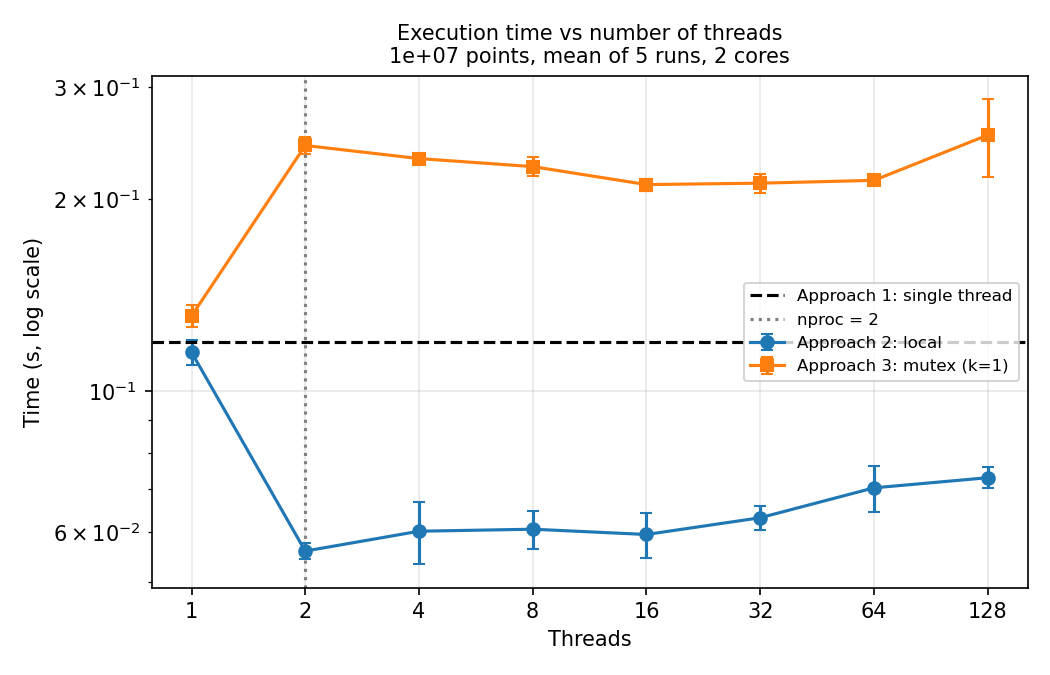
\includegraphics[width=\textwidth]{time.png}
  \caption{Thời gian chạy theo số luồng (thang log, thanh sai số là độ lệch chuẩn)}
  \label{fig:time}
\end{figure}
\begin{figure}[H]
  \centering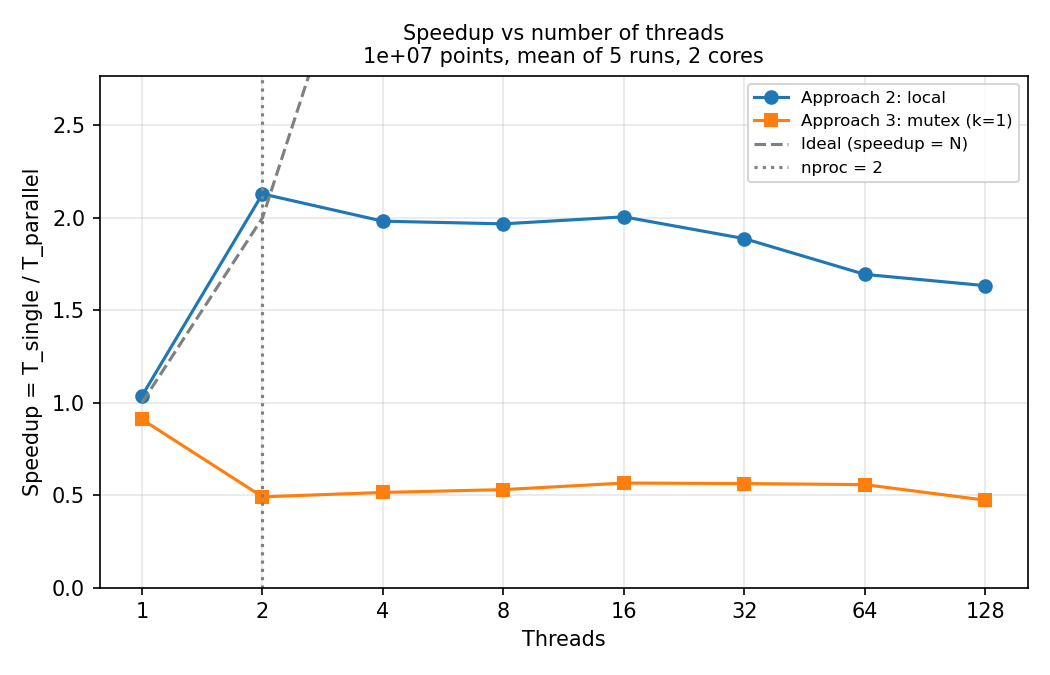
\includegraphics[width=\textwidth]{speedup.png}
  \caption{Speedup theo số luồng, so với đường lý tưởng $S=N$}
  \label{fig:speedup}
\end{figure}
\begin{figure}[H]
  \centering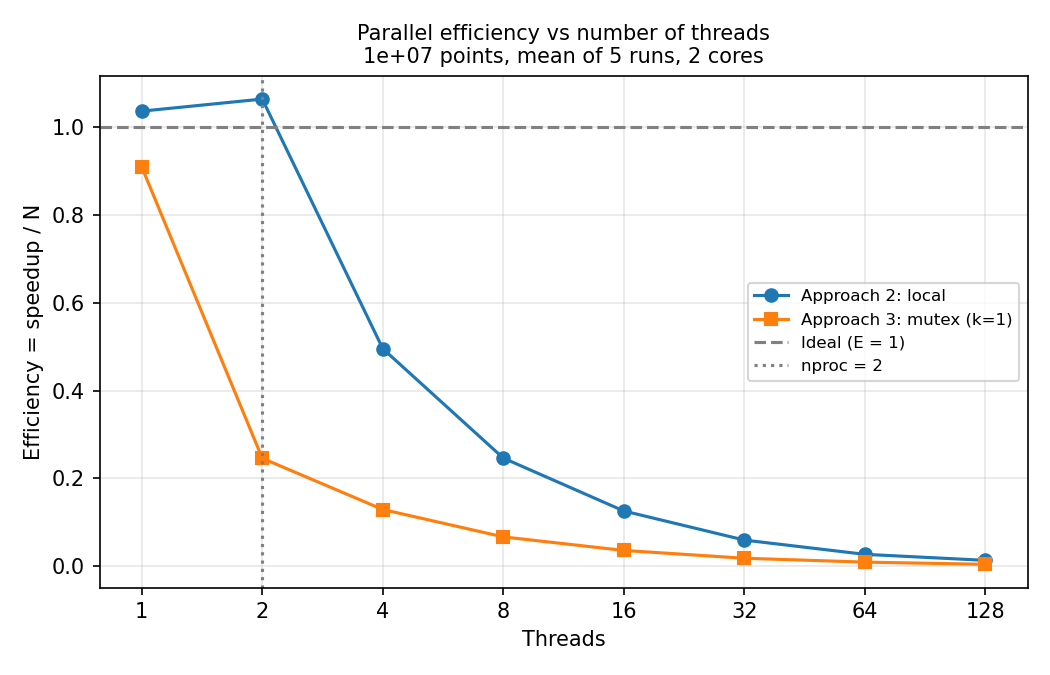
\includegraphics[width=\textwidth]{efficiency.png}
  \caption{Hiệu suất song song $E=S/N$}
  \label{fig:eff}
\end{figure}

\subsection{Độ chính xác của $\pi$}
\label{sec:pi}
Trong bảng thời gian, 5 lần chạy của một cấu hình dùng cùng seed 42 để cùng làm một khối việc, nên $\pi$ của 5 lần giống hệt nhau và chỉ thời gian thay đổi. Để xem $\pi$ dao động giữa các lần, \code{scripts/run\_precision.sh} chạy thêm 5 lần với 5 seed khác nhau, cách nhau 1000. Seed phải cách xa nhau vì luồng \code{tid} dùng seed \code{seed + tid}: hai lần chạy lệch nhau 1 seed sẽ dùng lại 3 trên 4 dãy số ngẫu nhiên, và không còn độc lập.

\begin{table}[H]
\centering
\caption{$\pi$ của 5 lần chạy với 5 seed khác nhau, $n=10^7$, $N=4$ (mutex dùng $k=1000$)}
\label{tab:pi_runs}
\begin{tabular}{cc|ccc}
\toprule
Lần & Seed & Một luồng & Cục bộ & Mutex \\
\midrule
1 & 42   & 3,140532 & 3,141520 & 3,141520 \\
2 & 1042 & 3,142388 & 3,141289 & 3,141289 \\
3 & 2042 & 3,140790 & 3,141713 & 3,141713 \\
4 & 3042 & 3,142003 & 3,141425 & 3,141425 \\
5 & 4042 & 3,141239 & 3,141278 & 3,141278 \\
\midrule
\multicolumn{2}{c|}{Trung bình} & 3,141390 & 3,141445 & 3,141445 \\
\multicolumn{2}{c|}{Độ lệch chuẩn} & 0,00079 & 0,00018 & 0,00018 \\
\multicolumn{2}{c|}{$|\bar\pi-\pi|$} & 0,00020 & 0,00015 & 0,00015 \\
\bottomrule
\end{tabular}
\end{table}

Mọi giá trị nằm trong khoảng 3,1403--3,1424, khớp sai số chuẩn $5{,}2\cdot10^{-4}$ của công thức~\eqref{eq:se}. Approach 3 cho đúng từng chữ số như Approach 2 ở cả 5 lần. \code{rand\_r} của glibc cho cùng một dãy số trên mọi máy, nên các giá trị $\pi$ ở đây không phụ thuộc máy đo.

\paragraph{Muốn đúng 5--6 chữ số thập phân.} Theo~\eqref{eq:se}, mỗi chữ số đúng thêm cần số điểm tăng 100 lần: 5 chữ số (sai số $\sim 3\cdot10^{-6}$) cần khoảng $3$--$5\cdot10^{11}$ điểm, 6 chữ số cần khoảng $4\cdot10^{13}$. \code{rand\_r} không làm được việc này: trạng thái của nó chỉ có 32 bit nên dãy số lặp lại sau tối đa $2^{32}$ số, tức khoảng $2\cdot10^9$ điểm. Kiểm định $\chi^2$ trên cặp $(x,y)$ liên tiếp với $10^7$ cặp cũng cho 8\,588, thấp hơn hẳn khoảng mong đợi [9\,724; 10\,278]: điểm của bộ sinh đồng dư tuyến tính rải \emph{đều hơn} ngẫu nhiên thật. Phân bố một chiều thì đạt ($\chi^2$ = 925{,}5 với 999 bậc tự do), và hai luồng seed 42 và 43 có hệ số tương quan $-0{,}0003$.

Vì vậy nhóm viết thêm \code{src/pi\_big.c}: cấu trúc giống Approach 2, nhưng mỗi luồng dùng bộ sinh 64 bit xoshiro256+ (chu kỳ $2^{256}-1$, khởi tạo bằng splitmix64 để các luồng không trùng dãy), số thực 53 bit và biến đếm 64 bit.

\begin{table}[H]
\centering
\caption{\code{pi\_big}, $N=4$, seed 42 (\code{results/precision.csv})}
\label{tab:precision}
\begin{tabular}{rlll}
\toprule
$n$ & $\hat\pi$ & $|\hat\pi-\pi|$ & $\sigma_{\hat\pi}$ \\
\midrule
$10^{7}$  & 3,1419652 & $3{,}7\cdot10^{-4}$ & $5{,}2\cdot10^{-4}$ \\
$10^{8}$  & 3,1416643 & $7{,}2\cdot10^{-5}$ & $1{,}6\cdot10^{-4}$ \\
$10^{9}$  & 3,1415584 & $3{,}4\cdot10^{-5}$ & $5{,}2\cdot10^{-5}$ \\
$10^{10}$ & 3,1415802 & $1{,}2\cdot10^{-5}$ & $1{,}6\cdot10^{-5}$ \\
$10^{11}$ & \textbf{3,14159}46 & $2{,}0\cdot10^{-6}$ & $5{,}2\cdot10^{-6}$ \\
$5\cdot10^{11}$ & \textbf{3,14159}60 & $3{,}3\cdot10^{-6}$ & $2{,}3\cdot10^{-6}$ \\
\bottomrule
\end{tabular}
\end{table}

Với $10^{11}$ điểm trở lên, kết quả đúng 5 chữ số thập phân 3,14159. Lần chạy $5\cdot10^{11}$ điểm mất \todo{thời gian trên máy đo, cột time\_sec của results/precision.csv} giây trên máy đo 4 vCPU. Sáu chữ số cần khoảng $4\cdot10^{13}$ điểm, tức gấp 80 lần lần chạy lớn nhất ở trên, khoảng vài giờ: nhóm không chạy trong khuôn khổ bài. Đây là giới hạn cố hữu của Monte Carlo: sai số chỉ giảm theo $1/\sqrt n$.

% =============================================================================
\section{Phân tích}
\subsection{A. Speedup không tuyến tính}
Định luật Amdahl (slide chương 4, \emph{Amdahl's Law}) giới hạn speedup của chương trình có phần tuần tự $s$:
\begin{equation}
  S(N)\le\frac{1}{s+(1-s)/N}.
\end{equation}
Vòng lặp Monte Carlo gần như song song hoàn hảo; phần tuần tự chỉ là tạo luồng, join và cộng gộp. Đo được $S(2)=1{,}87$ và $S(4)=3{,}58$, thấp hơn lý tưởng 2 và 4. Giải $S(4)=3{,}58$ theo Amdahl cho $s\approx 3{,}9\,\%$. Con số này lớn hơn phần tuần tự thật của chương trình, vì nó còn gánh những chi phí mà công thức Amdahl không mô hình hoá: các nhân của máy ảo do máy chủ định thời, nên có lúc một vCPU bị dừng; xung nhịp CPU có thể hạ khi nhiều nhân cùng bận; và join phải chờ luồng chậm nhất. Ngay ở $N=1$, Approach 2 chậm hơn Approach 1 khoảng 4\,\% (0,1066 so với 0,1028\,s), là chi phí tạo một luồng và join.

\subsection{B. Điểm bão hoà}
Các luồng chỉ thật sự chạy song song tới số nhân mà hệ điều hành định thời được, ở đây \code{nproc} = 4. Thời gian tốt nhất của Approach 2 là 0,0287\,s tại $N=4$, đúng bằng số vCPU. Từ 4 lên 8, 16, 32 luồng thời gian gần như không đổi (0,0287 $\to$ 0,0315\,s): thêm luồng không thêm nhân, các luồng chỉ chia nhau 4 nhân sẵn có theo lát thời gian. Đường cong này giống đồ thị mẫu của đề (máy 4 nhân, đỉnh ở 4 luồng).

\subsection{C. Quá tải luồng (oversubscription)}
Khi số luồng lớn hơn số nhân, bộ định thời (chương 5) cho từng luồng sẵn sàng chạy một lát thời gian theo lượt. Tổng thời gian CPU không đổi nên lượng việc có ích mỗi giây không tăng, trong khi mỗi luồng thêm vào kéo theo chi phí:
\begin{itemize}
  \item chuyển ngữ cảnh mỗi lần bộ định thời đổi luồng trên một nhân;
  \item cache và bộ dự đoán rẽ nhánh phải nạp lại sau mỗi lần đổi;
  \item thời gian tạo và join của từng luồng;
  \item luồng hoàn thành không đều: join chờ luồng cuối, nên một luồng bị tạm ngưng gần cuối làm chậm cả lần chạy.
\end{itemize}
Số đo cho thấy đúng điều đó: 32 luồng mất 0,0315\,s, 64 luồng 0,0465\,s (chậm hơn 62\,\% so với $N=4$). Độ lệch chuẩn cũng tăng vọt, từ $\le 0{,}002$\,s khi $N\le 32$ lên 0,012\,s ở $N=64$ và 0,010\,s ở $N=128$: thời gian chạy phụ thuộc vào thứ tự định thời, mỗi lần một khác. $N=128$ nhanh hơn $N=64$ một chút (0,0433 so với 0,0465\,s), nằm trong độ lệch chuẩn của hai điểm này nên không kết luận được gì.

\subsection{D. Chi phí đồng bộ}
Lệnh tăng \code{g\_inside} là vùng tranh chấp (critical section, chương 6): mỗi lúc chỉ một luồng được thực thi. Với $k=1$, mọi vòng lặp đều cần khoá:
\begin{itemize}
  \item \textbf{Tranh chấp.} Khi mutex rảnh, \code{pthread\_mutex\_lock} chỉ là một lệnh nguyên tử trong user space. Khi luồng khác đang giữ, luồng gọi phải ngủ trong kernel qua system call \code{futex}, và luồng nhả khoá phải gọi thêm một system call để đánh thức nó. Mỗi lần ngủ và thức là một lần chuyển ngữ cảnh, đắt hơn nhiều so với vài phép tính của một điểm Monte Carlo.
  \item \textbf{Tuần tự hoá.} Dù có bao nhiêu luồng, các lượt cộng vẫn diễn ra lần lượt từng cái, nên phần việc quan trọng của vòng lặp không nhanh lên được.
  \item \textbf{Chuyển cache line.} Mutex và biến đếm nằm ở vùng nhớ mà mọi nhân đều ghi. Mỗi lần lấy khoá, cache line đó phải chuyển sang nhân đang lấy, các nhân liên tục làm mất hiệu lực bản sao của nhau.
\end{itemize}
Ở $N=1$ (không có tranh chấp), riêng chi phí khoá và mở khoá đã là $0{,}1285-0{,}1028 = 0{,}026$\,s cho $10^7$ lượt, khoảng 2,6\,ns mỗi cặp. Ở $N=4$, Approach 3 mất 0,2838\,s so với 0,0287\,s của Approach 2: \textbf{chậm 9,9 lần}, và chậm gần 3 lần so với chạy một luồng. Từ $N=2$ trở đi thời gian gần như hằng số (0,27--0,30\,s): thêm luồng chỉ thêm người xếp hàng trước cùng một khoá.

\subsection{E. Hiệu suất song song}
$E(N)$ cho biết bao nhiêu phần năng lực của mỗi luồng thêm vào biến thành speedup có ích. Với Approach 2, $E$ giữ ở 0,90--0,96 khi $N\le 4$ (mỗi luồng có nhân riêng), rồi giảm gần đúng theo $4/N$ khi $N>4$ vì $S$ không tăng nữa: 0,44 ở $N=8$, 0,10 ở $N=32$, 0,019 ở $N=128$. Với Approach 3, khoá làm $E$ rơi ngay từ luồng thứ hai: 0,19 ở $N=2$ và 0,09 ở $N=4$.

% =============================================================================
\section{Thí nghiệm đánh đổi}
\subsection{Tần suất đồng bộ}
\label{sec:k}
Chạy Approach 3 với $N=4$ và $k$ = 1, 10, 100, 1\,000, 10\,000, 100\,000. Mỗi luồng giờ chỉ lấy khoá khoảng $n/(N k)$ lần thay vì mỗi điểm một lần, nên chi phí tranh chấp giảm theo $k$.

\begin{table}[H]
\centering
\caption{Approach 3 với $N=4$ theo $k$; Approach 2 cùng $N$ mất 0,0287\,s}
\label{tab:k}
\begin{tabular}{rrrr}
\toprule
$k$ & Số lần lấy khoá mỗi luồng & $T$ (s) & So với Approach 2 \\
\midrule
1       & 2\,500\,000 & 0,2838 & $\times$9,9 \\
10      & 250\,000    & 0,0800 & $\times$2,8 \\
100     & 25\,000     & 0,0330 & +15\,\% \\
1\,000  & 2\,500      & 0,0318 & +11\,\% \\
10\,000 & 250         & 0,0318 & +11\,\% \\
100\,000& 25          & 0,0304 & +6\,\% \\
\bottomrule
\end{tabular}
\end{table}

\begin{figure}[H]
  \centering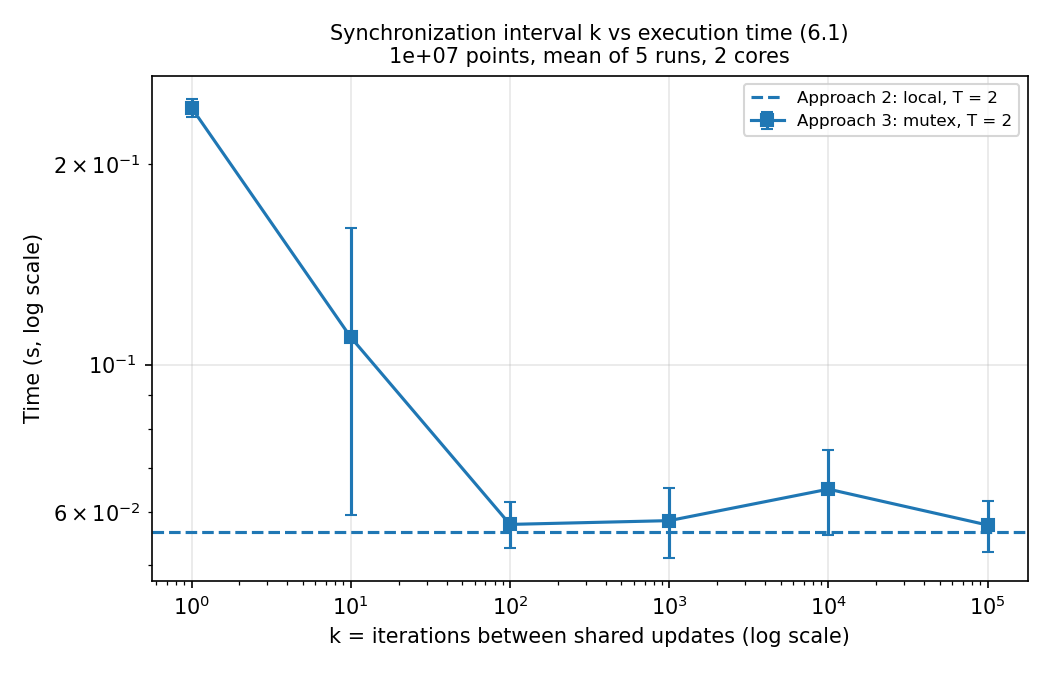
\includegraphics[width=\textwidth]{sync_k.png}
  \caption{Thời gian Approach 3 theo khoảng đồng bộ $k$ ($N=4$), đường ngang là Approach 2}
  \label{fig:k}
\end{figure}

Từ $k=100$, thời gian còn cách Approach 2 trong khoảng 6--15\,\%, chênh lệch cỡ độ lệch chuẩn của các điểm này (0,003--0,004\,s). Phần còn lại là phép chia lấy dư \code{(i + 1) \% k} ở mọi vòng lặp, Approach 2 không có. Kết luận: đồng bộ thưa đủ mức thì chi phí khoá gần như biến mất.

\subsection{Mở rộng số luồng}
Dải số luồng phủ ba vùng: ít hơn số nhân ($N<4$), bằng số nhân ($N=4$) và lớn hơn tới 128. Hình~\ref{fig:time} và~\ref{fig:speedup} cho đúng hình dạng dự kiến: thời gian giảm tới $N=4$, đi ngang tới $N=32$, rồi tăng ở $N=64$--128 do quá tải luồng (mục C).

\subsection{Tính cục bộ và tính dùng chung}
\begin{table}[H]
\centering
\caption{So sánh Approach 2 và Approach 3 ($k=1$)}
\label{tab:local_vs_shared}
\begin{tabularx}{\textwidth}{l|X|X}
\toprule
 & Approach 2 (cục bộ) & Approach 3 (dùng chung, $k=1$) \\
\midrule
Vùng tranh chấp & không có trong vòng lặp, chỉ bước cộng gộp sau join & lệnh tăng biến đếm, mỗi vòng một lần \\
Tranh chấp khoá & không & mọi luồng tranh một mutex \\
Tuần tự hoá & không trong lúc tính & mọi lượt cộng xếp hàng lần lượt \\
$T$ tại $N=4$ & 0,0287\,s & 0,2838\,s \\
\bottomrule
\end{tabularx}
\end{table}

% =============================================================================
\section{Các thực hành tốt rút ra}
Mỗi thực hành đi kèm một số đo của nhóm.
\begin{enumerate}
  \item \textbf{Đếm cục bộ, gộp một lần (map--reduce).} Ở $N=4$: 0,0287\,s so với 0,2838\,s khi dùng biến chung có khoá.
  \item \textbf{Số luồng bằng số nhân.} Speedup dừng ở $N=4$ = \code{nproc}; thêm luồng không nhanh hơn, quá nhiều luồng ($N=64$) còn chậm hơn 62\,\%.
  \item \textbf{Đồng bộ càng thưa càng tốt.} Với $k\ge 100$, bản dùng mutex chỉ chậm hơn bản không khoá 6--15\,\%.
  \item \textbf{Mỗi luồng một trạng thái sinh số ngẫu nhiên.} Dùng \code{rand\_r} với seed riêng; \code{rand()} có trạng thái chung sẽ xếp hàng các luồng sau một khoá ẩn.
  \item \textbf{Dữ liệu riêng của luồng không nằm chung cache line.} Đếm trong biến stack, không trong \code{count[tid]} (false sharing).
  \item \textbf{Đo thời gian đúng cách.} Dùng \code{CLOCK\_MONOTONIC}, không dùng \code{clock()}; chạy nhiều lần, báo trung bình và độ lệch. Ở $N\ge 64$ độ lệch chuẩn tăng gấp 5 lần, một lần đo duy nhất sẽ cho kết luận sai.
  \item \textbf{Kiểm tra đúng sai, không chỉ tốc độ.} Cùng seed thì \code{inside} phải giống nhau giữa các approach; bỏ khoá thì mất khoảng 78\,\% lượt cộng.
  \item \textbf{Chọn bộ sinh số ngẫu nhiên đủ cho độ chính xác cần.} \code{rand\_r} 32 bit lặp lại sau $\sim 2\cdot10^9$ điểm; muốn 5 chữ số thập phân thì cần bộ sinh 64 bit và $\ge 10^{11}$ điểm.
\end{enumerate}

% =============================================================================
\section{Kết luận}
Ước lượng song song của bài toán gần như không có phần tuần tự đạt speedup 3,58 trên 4 vCPU, bão hoà đúng tại số nhân và chậm lại khi quá tải luồng. Khoá mutex ở mọi vòng lặp làm chương trình chậm hơn cả một luồng; đồng bộ thưa ($k\ge 100$) xoá gần hết chi phí đó. Về độ chính xác, $10^7$ điểm cho khoảng 3 chữ số thập phân đúng; 5 chữ số cần $10^{11}$ điểm và một bộ sinh số 64 bit.

% =============================================================================
\section*{Sử dụng công cụ AI}
\addcontentsline{toc}{section}{Sử dụng công cụ AI}
Theo quy định của đề cương môn học: \todo{nhóm liệt kê công cụ AI đã dùng và dùng vào việc gì, ví dụ Claude Code dùng để lập kế hoạch chia việc, viết script đo/vẽ, review pull request và soạn báo cáo}. Mọi số liệu trong báo cáo đến từ việc chạy mã của nhóm trên máy đo.

\end{document}
